% !TEX root = main.tex

%%%%%%%%%%%%%%%%%%%%%%%%%%%%%%%%%%%%%%%%%%%%%%%%%%%%%%%%%%%%%%%%%%%%%%%%%%%%%%%%%%%%%%%%%%%%%%%%
\section{理論}
%%%%%%%%%%%%%%%%%%%%%%%%%%%%%%%%%%%%%%%%%%%%%%%%%%%%%%%%%%%%%%%%%%%%%%%%%%%%%%%%%%%%%%%%%%%%%%%%
図1に示す2つの端子対からなる回路を考える.入力端子対$1,1'$の電圧,電流$V_1$,$I_1$は,
出力端子対$2,2'$の電圧,電流$V_2$,$I_2$により
$$
\left[\begin{array}{c}
V_1 \\
I_1
\end{array}\right]=\left[\begin{array}{ll}
A & B \\
C & D
\end{array}\right]\left[\begin{array}{c}
V_2 \\
I_2
\end{array}\right]
$$
と表される.この式中の2行2列の行列
$$
\left[\begin{array}{ll}A & B \\ C & D\end{array}\right]
$$
をF行列とよび,この行列の各要素$A,B,C,D$を4端子定数とよぶ.4端子定数$A$は出力端子対$2,2'$を開放した時の入力電圧$V_1$と出力電圧$V_2$の比
$$
A=\left.\frac{V_1}{V_2}\right|_{I_2=0}
$$
と定義される.また,$B$は出力端子対$2,2'$を短絡した時の入力電圧$V_1$と出力電流$I_2$の比
$$
B=\left.\frac{V_1}{I_2}\right|_{V_2=0}
$$
であり,$C$は出力端子対$2,2'$を開放した時の入力電流$I_1$と出力電圧$V_2$の比
$$
C=\left.\frac{I_1}{V_2}\right|_{I_2=0}
$$
であり,$D$は出力端子対$2,2'$を短絡した時の入力電流$I_1$と出力電流$I_2$の比
$$
D=\left.\frac{I_1}{I_2}\right|_{V_2=0}
$$
である.


図2のように2端子対回路を縦続接続すると,全体の回路のF行列は各々の回路のF行列の積で表される.
すなわち

$$
\left[\begin{array}{l}
V_1 \\
I_1
\end{array}\right]=\left[\begin{array}{ll}
A & B \\
C & D
\end{array}\right]\left[\begin{array}{c}
V_3 \\
I_3
\end{array}\right]
$$

とすると、

$$
\left[\begin{array}{l}
V_1 \\
I_1
\end{array}\right]=\left[\begin{array}{ll}
A_1 & B_1 \\
C_1 & D_1
\end{array}\right]\left[\begin{array}{l}
V_2 \\
I_2
\end{array}\right]
$$

$$
\left[\begin{array}{c}
V_2 \\
I_2
\end{array}\right]=\left[\begin{array}{ll}
A_2 & B_2 \\
C_2 & D_2
\end{array}\right]\left[\begin{array}{l}
V_3 \\
I_3
\end{array}\right]
$$

より

$$
\left[\begin{array}{ll}
A & B \\
C & D
\end{array}\right]=\left[\begin{array}{ll}
A_1 & B_1 \\
C_1 & D_1
\end{array}\right]\left[\begin{array}{ll}
A_2 & B_2 \\
C_2 & D_2
\end{array}\right]
$$

と表される.


$R,L,C,M$以外の素子を含まない回路では,F行列の行列式$AD-BC$の値は1となる.
また,入力端子と出力端子を入れ替えた回路のF行列は,AとDを入れ替えたものとなる.

\begin{figure}
    \begin{center}
        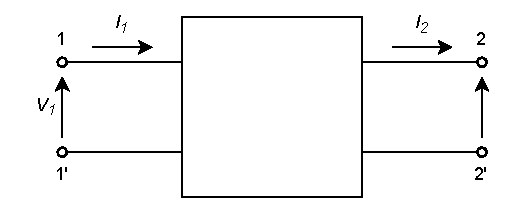
\includegraphics[]{figure1.drawio.pdf}
        \caption{2端子対回路}
    \end{center}
\end{figure}

\begin{figure}
    \begin{center}
        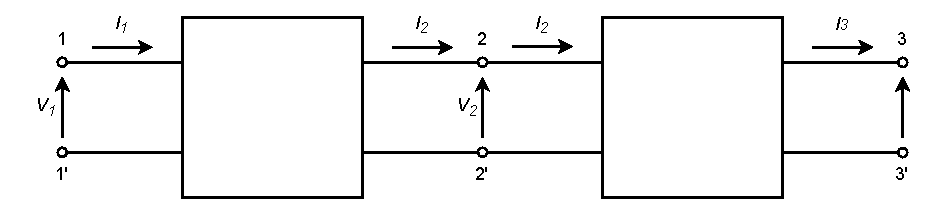
\includegraphics[]{figure2.drawio.pdf}
        \caption{2端子対回路の縦続接続}
    \end{center}
\end{figure}